\begin{frame}[fragile]{MiniBrass}

\begin{center}

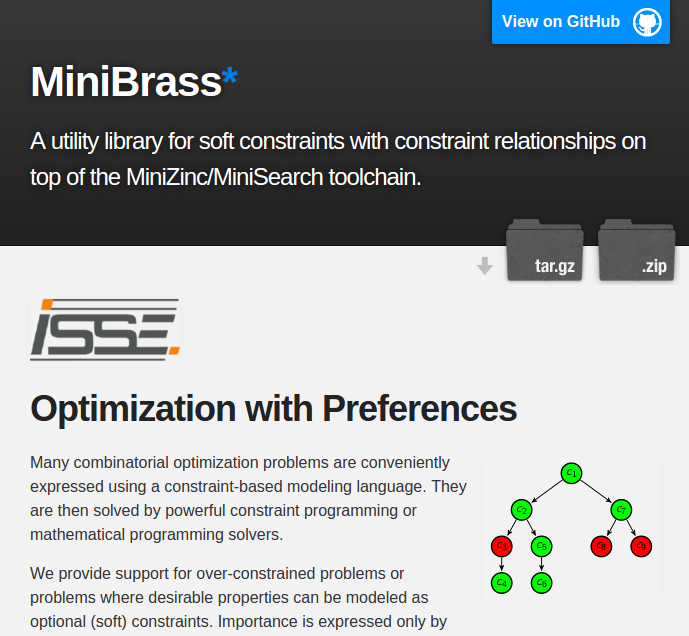
\includegraphics[width=.5\textwidth]{img/minibrass.png}

\vspace*{2ex}

\url{http://isse-augsburg.github.io/minibrass/}

\end{center}

\end{frame}

\begin{frame}[fragile]{MiniBrass: HelloWorld}
\begin{columns}[onlytextwidth,T]
    
    \begin{column}{.40\textwidth}
          
    \hSecond{Base model (MiniZinc)}
    \begin{lstlisting}
include "hello_o.mzn"; 
include "soft_constraints/
   pvs_gen_search.mzn"; 
% the basic, "classic" CSP 
set of int: DOM = 1..3;

var DOM: x; var DOM: y; 
var DOM: z;
% add. *hard* constraints
% e.g. constraint x < y;

solve search pvs_BAB();
\end{lstlisting}
    \end{column}
    
    \begin{column}{.55\textwidth}
  	\hFirst{Preference model (MiniBrass)} 
  	\begin{lstlisting}
PVS: cr1 = 
  new ConstraintRelationships("cr1") {
   soft-constraint c1: 'x + 1 = y';
   soft-constraint c2: 'z = y + 2';
   soft-constraint c3: 'x + y <= 3';
   
   crEdges : '[| mbr.c2, mbr.c1 | 
                  mbr.c3, mbr.c1 |]';
   useSPD: 'true' ;
}; 

solve cr1;
\end{lstlisting}

    \end{column}
  \end{columns}
  \pause
  \begin{verbatim}
Solution:  x = 1; y = 2; z = 1
Valuations:  mbr_overall_cr1 = {c2}
----------
==========
  \end{verbatim}
  \begin{textblock*}{3cm}[1,1](\textwidth+0.5cm,\textheight-0.3cm)
%\textblockcolour{issegrey!20}
\begin{center}
\begin{tikzpicture}[auto,
                    ->,>=stealth',shorten >=1pt,thick,
                    node distance=.7cm,inner sep=2pt,
                    constraint/.style={circle,fill=black!15,draw,font=\sffamily\small}]
\node[constraint node] (1) at (0, 0)                   {$\mathrm{c}_1$};
\node[constraint node] (2) at ($ (1) + (-0.8, -0.8) $) {$\mathrm{c}_2$};  
\node[constraint node] (3) at ($ (1) + ( 0.8, -0.8) $) {$\mathrm{c}_3$};  
%  
\path[every node/.style={font=\sffamily\tiny}]
  (2) edge (1)
  (3) edge (1)
  ;
  

\end{tikzpicture}
\end{center}
\end{textblock*}
\end{frame}


\tikzset{onslide/.code args={<#1>#2}{%
  \only<#1>{\pgfkeysalso{#2}}
}}
\tikzstyle{highlight}=[isseorange,ultra thick]
\tikzstyle{highlight2}=[CornflowerBlue,ultra thick]
\begin{frame}[fragile]{Constraint Optimization with Preferences}
The partially-ordered valuation space



\begin{figure}[!t]
\begin{center}
\begin{tikzpicture}[scale=0.77,auto]

% single PVS
\node (bot) at (0,0) {\alert{$\bot = \{c_1, c_2, c_3 \}$}};
\node (c1c2) at (-2,1) {\alert<2->{$\{c_1, c_2\}$}};
\node (c2c3) at (0,2) {$\{c_2, c_3\}$};
\node (c1c3) at (2,1) {$\{c_1, c_3\}$};

\node (c1) at (0,3) {\alert<3->{$\{c_1\}$}};
\node (c2) at (-2,4) {\alert<4->{$\{c_2\}$}};
\node (c3) at (2,4) {$\{c_3\}$};
%\node (a) at (-1,0.5) {$a$};
%\node (b) at (-1,1.5) {$b$};
%\node (c) at (1,1) {$c$};
\node (top) at (0,5) {$\top = \emptyset$};

\node[text width=2cm] (verb) at (4,0) {     };
\path[-]
(bot) edge[onslide={<2->{highlight}}] (c1c2)
      edge (c2c3)
      edge (c1c3)
(c1c2) edge (c2c3)
(c1c3) edge (c2c3)
(c1c3) edge (c1)
(c1c3) edge (c3)
(c2c3) edge (c2)
(c2c3) edge (c3)
(c1c2) edge[onslide={<3->{highlight}}] (c1)
(c1c2) edge (c2)
(c1) edge[onslide={<4->{highlight}}] (c2)
(c1) edge (c3)
(c2) edge (top)
(c1) edge (top)
(c3) edge (top)
      ;
%(a) edge (b)
%(b) edge (top)
%(bot) edge (c)
%(c) edge (top)
;

\end{tikzpicture}
\end{center}
\label{fig:nosuprema}
\end{figure}
\begin{lstlisting}
function ann: pvs_BAB() =
       repeat(
           if next() then 
                 print("Intermediate solution:") /\ print() /\
                 commit() /\ postGetBetter()
           else break endif       );
\end{lstlisting}
\begin{textblock*}{2.5cm}[1,1](\textwidth-8.8cm,\textheight-4.03cm)
\begin{tikzpicture}[auto,
                    ->,>=stealth',shorten >=1pt,thick,
                    node distance=.7cm,inner sep=2pt,
                    constraint/.style={circle,fill=black!15,draw,font=\sffamily\small}]
\node[constraint node] (1) at (0, 0)                   {$\mathrm{c}_1$};
\node[constraint node] (2) at ($ (1) + (-0.8, -0.8) $) {$\mathrm{c}_2$};  
\node[constraint node] (3) at ($ (1) + ( 0.8, -0.8) $) {$\mathrm{c}_3$};  
%  
\path[every node/.style={font=\sffamily\tiny}]
  (2) edge (1)
  (3) edge (1)
  ;
  

\end{tikzpicture}
\begin{Verbatim}[fontsize=\small]
c1: 'x + 1 = y';
c2: 'z = y + 2';
c3: 'x + y <= 3';   
\end{Verbatim}
\end{textblock*}

\begin{textblock*}{4cm}[1,1](\textwidth+0.5cm,\textheight-3.03cm)

\onslide<2->{

{ \tt  \small
x = 1; y = 1; z = 1 \newline
Valuation = \{c1,c2\}
}
}

\onslide<3->{
{ \tt  \small
----------

x = 1; y = 1; z = 3 \newline
Valuation = \{c1\}
}
}


\onslide<4->{
{ \tt  \small
----------

x = 1; y = 2; z = 1 \newline
Valuations = \{c2\}

----------

==========

}
}
\end{textblock*}
\end{frame}

\begin{frame}{Is that all?}
\begin{itemize}
\item Does MiniBrass only support Constraint Relationships? \pause 
\item Of course not, there other ways to express preferences:
\begin{itemize} \pause 
\item[-] Weights/costs/penalties (violation of a constraint leads to $5$ penalty points) \pause 
\item[-] Fuzzy satisfaction degrees, ranging from $0$ (not acceptable) to $1$ (maximally satisfied) \pause 
\item[-] Probabilities (``if I leave at 8am, the probability of actually meeting my deadline is 40\%'') \pause 
\item[-] \ldots
\end{itemize}

\vspace*{2ex}
\item What is the common underlying abstract data type?
\item What's up with \texttt{PVS: cr = new ConstraintRelationship}
\end{itemize}
\end{frame}


% block styles
\tikzstyle{sensor}=[draw, fill=blue!20, text width=5em, 
    text centered, minimum height=2.5em,drop shadow]    
    
\tikzstyle{alg} = [sensor, text width=5em, fill=isseorange!20, 
    minimum height=13em, rounded corners, drop shadow]
\tikzstyle{constraint}=[draw, circle, fill=issegrey!20, text width=1.2em, 
    text centered, minimum height=1.5em,drop shadow]
\tikzstyle{domainstore} = [alg, text width=5em, fill=isseorange!40, 
    minimum height=4em, rounded corners]
\tikzstyle{goodc} = [ForestGreen, font=\bfseries]
\tikzstyle{badc} = [Red, font=\bfseries]
\tikzstyle{okayc} = [LimeGreen, font=\bfseries]
        
\tikzset{
vecArrow/.style={
  thick
  }
}

\tikzset{
    mn/.style={rectangle,rounded corners,draw=black, top color=isseorange!5, bottom color=isseorange!30,
                   very thick, inner sep=\myinnersep*1em, minimum size=3em, text centered, outer sep=0, align=center},
    innernode/.style={mn, text width=3cm,  minimum height=1.5cm,
                      top color=issegrey!20, bottom color=issegrey!60},
    emphnode/.style={innernode, top color=isseorange!30, bottom color=isseorange!70}
}

% Define distances for bordering
\def\blockdist{2.3}
\def\edgedist{2.5}

  \tikzset{
    invisible/.style={opacity=0},
    visible on/.style={alt={#1{}{invisible}}},
    alt/.code args={<#1>#2#3}{%
      \alt<#1>{\pgfkeysalso{#2}}{\pgfkeysalso{#3}} % \pgfkeysalso doesn't change the path
    },
  }
  
%\begin{frame}{Traditional Constraint Solving}
%\begin{center}
%\begin{tikzpicture}
%% First row:
% \node (search) [alg]  {Search \phantom{$x = 5$} };
% \path (search.east)+(4.6,0) node (propag) [alg,text width =12em]  {};
% \node[below right] at (propag.north west) {Constraint Store $C$};
% 
% \path (propag.west)+(0.8,-1.2) node (c1) [constraint] {$c_1$}; 
% \path (propag.west)+(1.1,-0.2) node (c2) [constraint] {$c_2$}; 
% \path (propag.west)+(2.0,0.4) node (c3) [constraint] {$c_3$}; 
% \path (propag.west)+(3.2,0.7) node (c4) [constraint] {$c_4$};
%  
% \path (propag.east)+(-1.2,-1.2) node (domainstore) [domainstore] {Domain Store $(D_x)_{x \in X}$}; 
% 
% \path [draw,vecArrow, ->] ([yshift=-2em]search.north east) -- node [above,visible on=<2->] {$x\gets5$} ([yshift=-2em]propag.north west);
% \path [draw,vecArrow, <-] ([yshift=2em]search.south east) -- node [above,goodc,visible on=<4->] {$\top$} ([yshift=2em]propag.south west);
% 
% \path [draw, vecArrow, <->] (c1.east) -- node [below,visible on=<3->,goodc] {$\top$} (domainstore.west) ;
% \path [draw,vecArrow, <->] (c2.330) -- node [above right,visible on=<3->,goodc] {$\top$} (domainstore.150) ;
% \path [draw,vecArrow, <->] (c3.290) -- node [right,visible on=<3->,goodc] {$\top$} (domainstore.120) ;
% \path [draw,vecArrow, <->] (c4.south) -- node [right,visible on=<3->,goodc] {$\top$} (domainstore.68) ;
%\end{tikzpicture}
%\end{center}
%\onslide<0>{
%\begin{columns}[c] % contents are top vertically aligned
%     \begin{column}[c]{7cm} % each column can also be its own 
%\begin{itemize}
%\item A set of satisfaction degrees, $\mathbb{B} = \{ \bot, \top \}$
%\item A combination operation $\wedge$
%\item A neutral element $\top$
%\item A partial ordering $(\mathbb{B}, \leq_\mathbb{B})$ with $\top <_\mathbb{B} \bot$ 
%\end{itemize}
%\end{column}
%     \begin{column}[c]{4.5cm} 
%     \end{column} 
%\end{columns}
%}
%
%\end{frame}

\begin{frame}{Traditional Constraint Solving}
\begin{center}
\begin{tikzpicture}
% First row:
 \node (search) [alg]  {Search $x = 5$};
 \path (search.east)+(4.6,0) node (propag) [alg,text width =12em]  {};
 \node[below right] at (propag.north west) {Constraint Store $C$};
 
 \path (propag.west)+(0.8,-1.2) node (c1) [constraint] {$c_1$}; 
 \path (propag.west)+(1.1,-0.2) node (c2) [constraint] {$c_2$}; 
 \path (propag.west)+(2.0,0.4) node (c3) [constraint] {$c_3$}; 
 \path (propag.west)+(3.2,0.7) node (c4) [constraint] {$c_4$};
  
 \path (propag.east)+(-1.2,-1.2) node (domainstore) [domainstore] {Domain Store $(D_x)_{x \in X}$}; 
 
 \path [draw,vecArrow, ->] ([yshift=-2em]search.north east) -- node [above,visible on=<2->] {$y \gets 4$} ([yshift=-2em]propag.north west);
 \path [draw,vecArrow, <-] ([yshift=2em]search.south east) -- node [below,badc,visible on=<4->] {$\bot$} ([yshift=2em]propag.south west);
 
 \path [draw, vecArrow, <->] (c1.east) -- node [below,visible on=<3->,badc] {$\bot$} (domainstore.west) ;
 \path [draw,vecArrow, <->] (c2.330) -- node [above right,visible on=<3->,goodc] {$\top$} (domainstore.150) ;
 \path [draw,vecArrow, <->] (c3.290) -- node [right,visible on=<3->,goodc] {$\top$} (domainstore.120) ;
 \path [draw,vecArrow, <->] (c4.south) -- node [right,visible on=<3->,goodc] {$\top$} (domainstore.68) ;
\end{tikzpicture}
\end{center}
\onslide<5->{
\begin{columns}[c] % contents are top vertically aligned
     \begin{column}[c]{8cm} % each column can also be its own 
\begin{itemize}
\item A set of satisfaction degrees, $\mathbb{B} = \{ \bot, \top \}$
\item A combination operation $\wedge$
\item A neutral element $\top$
\item A partial ordering $(\mathbb{B}, \leq_\mathbb{B})$ with $\top <_\mathbb{B} \bot$ 
\end{itemize}
   \end{column} 
     \begin{column}[c]{4.5cm} 
     \end{column} 
\end{columns}
}
\end{frame}

\begin{frame}{Soft-Constraint-Solving}
\begin{center}
\begin{tikzpicture}
% First row:
 \node (search) [alg]  {Search $x = 5$};
 \path (search.east)+(4.6,0) node (propag) [alg,text width =12em]  {};
 \node[below right] at (propag.north west) {Constraint Store $C$};
 
 \path (propag.west)+(0.8,-1.2) node (c1) [constraint] {$c_1$}; 
 \path (propag.west)+(1.1,-0.2) node (c2) [constraint] {$c_2$}; 
 \path (propag.west)+(2.0,0.4) node (c3) [constraint] {$c_3$}; 
 \path (propag.west)+(3.2,0.7) node (c4) [constraint] {$c_4$};
  
 \path (propag.east)+(-1.2,-1.2) node (domainstore) [domainstore] {Domain Store $(D_x)_{x \in X}$}; 
 
 \path [draw,vecArrow, ->] ([yshift=-2em]search.north east) -- node [above,visible on=<2->] {$y \gets 4$} ([yshift=-2em]propag.north west);
 \path [draw,vecArrow, <-] ([yshift=2em]search.south east) -- node [below,okayc,visible on=<4->] {$4$} ([yshift=2em]propag.south west);
 
 \path [draw, vecArrow, <->] (c1.east) -- node [below,visible on=<3->,okayc] {$4$} (domainstore.west) ;
 \path [draw,vecArrow, <->] (c2.330) -- node [above right,visible on=<3->,goodc] {$0$} (domainstore.150) ;
 \path [draw,vecArrow, <->] (c3.290) -- node [right,visible on=<3->,goodc] {$0$} (domainstore.120) ;
 \path [draw,vecArrow, <->] (c4.south) -- node [right,visible on=<3->,goodc] {$0$} (domainstore.68) ;
\end{tikzpicture}
\end{center}
\onslide<5->{
\begin{columns}[c] % contents are top vertically aligned
     \begin{column}[c]{8cm} % each column can also be its own environment
    \begin{itemize}
\item A set of satisfaction degrees, e.g., $\{ 0, \ldots, k \}$
\item A combination operation $+$
\item A neutral element $0$
\item A partial ordering $(\mathbb{N}_0, \geq)$ with $0$ as top
\end{itemize}
   \end{column} \pause
     \begin{column}[c]{4.5cm} 
    %    Eine \cemph{valuation structure}~\cite{Schiex1995valued}, wenn die Ordnung total ist, sonst eine  \cemph{partial valuation structure}~\cite{Gadducci2013} (PVS).
     \end{column}
\end{columns}
    
}
\end{frame}

\begin{frame}{Partial Valuation Structures}
Underlying \alert{abstract data type}:
Partial valuation structure %\emph{(= partially ordered, commutative monoid)}
\begin{itemize}
\item $(M, \cdot_M, \varepsilon_M, \leq_M)$ 
\item $m \cdot_m \varepsilon_M = m$
\item $m \leq_M \varepsilon_M$
\item $m \leq_M n \rightarrow m \cdot_M o \leq_M n \cdot_M o$
\end{itemize}

\vspace*{2ex}

\begin{columns}[onlytextwidth,T]
    
    \begin{column}{.7\textwidth}
          
    \hSecond{Abstract}
    
    \begin{itemize}
    \item $M$ \ldots elements
    \item $\cdot_M$ \ldots combination function
    \item $\varepsilon_M$ \ldots neutral, ``best'' element
    \item $\leq_M$ \ldots ordering, left``worse''
    \end{itemize}
    \end{column}
    
    \begin{column}{.3\textwidth}
  	\hFirst{Concrete}  
  	 \begin{itemize}
    \item $\{0, \ldots, k \}$ 
    \item $+_k$
    \item $0$ 
    \item $\geq$
    \end{itemize}
    \end{column}
  \end{columns}

  \vspace*{2ex}
  
\begin{textblock*}{4.cm}[1,1](\textwidth-0.5cm,\textheight-4.63cm)

\includegraphics[width=\textwidth]{img/scales.jpg}
\end{textblock*}
  \hfill \emph{\cite{Gadducci2013,SchiendorferPvs2015}}
\end{frame}


\tikzset{
    process/.style={rectangle,rounded corners,draw=black, top color=isseorange!5, bottom color=isseorange!30},
    file/.style={rectangle,draw=black}
}
\begin{frame}{MiniBrass: Workflow} \small

\vspace*{-2ex}
\alert{Architecture}

\begin{center}
\vspace*{-10ex}
\begin{tikzpicture}[>=stealth,auto,every node/.style={
anchor=base,
text depth=.5ex,
text height=2ex,
minimum height=2ex,
align=center,
circle,
minimum width=1em}]
\matrix (magic) [nodes in empty cells, ampersand replacement=\&,row sep=0.5cm,column sep=0.5cm]
{
\node{}; \&\node[draw, file,isseorange,thick](mbrlibs){\texttt{mbrlibs.mzn}}; \& \& \node[draw, file,isseorange,thick](types){\texttt{types.mbr}}; \\
\node {};\& \node[draw, file,CornflowerBlue,thick](mbr){\texttt{prefs.mbr}};   \& \& \node[draw, isseorange,thick,process](mbr2mzn){\texttt{mbr2mzn}}; \\
\node {};\& \& \& \node[draw, file,isseorange,thick](compiledMzn){\emph{prefs\_o.mzn}}; \\
%    \&  \&  \node(inv){}; \&  \\
\node {};\& \node[draw, file,CornflowerBlue!80](f1){\texttt{model.mzn}}; \& \& \node[draw, process](mzn2fzn){\texttt{mzn2fzn}}; \& \& \node[draw, file](output){\emph{output}};  \\
%    \&  \&  \node(inv){}; \&  \\
\node {};\& \node[draw, file,CornflowerBlue!80](mod){\texttt{data.dzn}}; \& \&  \\
\node {};\& \node[draw, file](mznlibs){\texttt{mznlibs.mzn}};\& \& \node[draw, file](fzn){\texttt{compiled.fzn}}; \& \& \node[draw, process](solve){\texttt{solve}};  \\
\node {};\& \& \\
};

\draw[dashed,->] (f1) -- (mzn2fzn);
\draw[dashed,->] (mbr) -- (mbr2mzn);
\draw[dashed,->] (mod) -- (mzn2fzn);
\draw[dashed,-] (types) -- (mbrlibs);
\draw[dashed,-] (types) -- (mbr);
%\draw[dashed,->] (mbrlibs) -- (mzn2fzn);
%\draw[dashed] (mbrlibs) -- (mbr);
\draw[dashed,->] (compiledMzn) -- (mzn2fzn);
\draw[dashed,->] (mznlibs) -- (mzn2fzn);
\draw[dashed,->] (fzn) -- (solve);
\draw[->] (mbr2mzn) -- (compiledMzn);

\draw[->] (mzn2fzn) -- (fzn);
\draw[->] (solve) -- (output);
%\draw[dashed] (globals) -- (inv);

%\onslide<4->{  
%\node[overlay,align=left,rectangle callout,%
%      callout absolute pointer=(mbrlibs.west),fill=CornflowerBlue!50] at (-4.5,5) {PVS-Prädikate};}

\onslide<4->{  
\node[overlay,align=left,rectangle callout,%
      callout absolute pointer=(mbrlibs.north),fill=isseorange!50] at (-3,7.5) {Implemented functions and predicates};}
            
\onslide<2->{  
\node[overlay,align=left,rectangle callout,%
      callout absolute pointer=(types.north),fill=isseorange!50] at (2,7.5) {PVS type definitions};} 
     
\onslide<3->{  
\node[overlay,align=left,rectangle callout,%
      callout absolute pointer=(mbr.west),fill=CornflowerBlue!50] at (-3.7,4.5) {PVS instances, combinations};} 
     
\end{tikzpicture}
\end{center}
\vspace*{-25ex}

\end{frame}

